\documentclass[UTF8]{ctexart}

\usepackage{amsmath,amssymb}
\usepackage[a4paper,margin=18mm]{geometry}
\usepackage{enumitem}
\usepackage{fancyhdr}
\usepackage{lastpage}

% TikZ for the schematic figure in Q11
\usepackage{tikz}
\usetikzlibrary{calc,angles,quotes}

\usepackage[a4paper,margin=18mm]{geometry}
\usepackage{xcolor}
\usepackage{tikz}
\usepackage{pgfplots}
\pgfplotsset{compat=1.18}

\setlength{\parindent}{2em}
\setlength{\parskip}{0.4em}

\usepackage{tikz}
\usetikzlibrary{calc,intersections,angles,quotes}

\begin{document}
	% （将以下内容直接粘贴到你的 LaTeX 正文中即可；如需编译中文，请使用 ctex 模板）
	
	\section{射影几何与极点极线理论（笔记版）}
	
	\subsection{学习目标}
	本节围绕圆/圆锥曲线命题中常见的“高级但可落地”的工具展开：
	\begin{itemize}
		\item 交比（cross ratio）的定义、计算与不变性；
		\item 调和点列/调和线束（harmonic division / harmonic pencil）；
		\item 圆锥曲线的极点--极线（pole--polar）对应与核心定理（尤其是 La Hire 定理）；
		\item 把“切线、弦、交点、共线、共点”类结论统一到一套射影语言下，服务于圆锥曲线题的证明与构造。
	\end{itemize}
	
	\subsection{射影几何的基本语言（最少必需版）}
	\paragraph{（1）齐次坐标与直线}
	射影平面中点可用齐次坐标表示为
	\[
	P=(x:y:z),\qquad (x,y,z)\neq (0,0,0),
	\]
	且 $(x:y:z)\sim (\lambda x:\lambda y:\lambda z)$（$\lambda\neq 0$）表示同一点。
	直线可写为
	\[
	\ell:\ ax+by+cz=0.
	\]
	点 $P$ 在直线 $\ell$ 上，当且仅当把 $P$ 代入上式成立。
	
	\paragraph{（2）“无穷远点/无穷远直线”的直观}
	欧氏平面中“平行线不相交”，射影几何中把它们的交点补到“无穷远”，从而许多命题具有更统一的表述（例如把相交与平行视为同一种现象）。
	
	\subsection{交比：定义、性质与不变性}
	\paragraph{（1）四点共线的交比}
	设 $A,B,C,D$ 是同一直线上的四点，使用有向线段，定义交比为
	\[
	(A,B;C,D)=\frac{\overrightarrow{CA}/\overrightarrow{CB}}{\overrightarrow{DA}/\overrightarrow{DB}}
	=\frac{\overrightarrow{CA}\cdot \overrightarrow{DB}}{\overrightarrow{CB}\cdot \overrightarrow{DA}}.
	\]
	在坐标轴上（把直线参数化为实数 $a,b,c,d$），也可写为
	\[
	(A,B;C,D)=\frac{(c-a)(d-b)}{(c-b)(d-a)}.
	\]
	
	\paragraph{（2）射影变换下的交比不变}
	交比是射影不变量：任意射影变换（包括透视投影、中心投影的复合）都保持交比不变。
	因此，许多“比值”问题可以先做射影化简，再还原。
	
	\paragraph{（3）六值性质（了解即可）}
	对四点重排会得到至多 $6$ 个不同数值（虽然共有 $4!=24$ 种排列）。
	
	\subsection{调和点列与调和线束}
	\paragraph{（1）调和点列}
	若
	\[
	(A,B;C,D)=-1,
	\]
	则称 $(A,B;C,D)$ 构成\textbf{调和点列}，并称 $D$ 为 $C$ 关于 $(A,B)$ 的\textbf{调和共轭点}（或称 $C,D$ 为关于 $A,B$ 的调和共轭）。
	
	\paragraph{（2）调和线束}
	设 $P$ 为平面内一点，四条射线 $PA,PB,PC,PD$ 构成线束。
	若 $(A,B;C,D)=-1$（其中 $A,B,C,D$ 是该线束与任意截线的交点），则称 $P(A,B,C,D)$ 为\textbf{调和线束}。
	
	\paragraph{（3）关键引理：投影保持交比}
	若从一点作中心投影把一条直线上的四点投影到另一条直线上，则交比保持不变。
	这条引理是把“图形构造”与“交比计算”连接起来的桥梁。
	
	\subsection{圆锥曲线的极点--极线（Pole--Polar）}
	以下在圆锥曲线（特别是圆）背景下使用。
	
	\paragraph{（1）外点的极线（从切线出发的定义）}
	给定圆（或一般圆锥曲线）$\mathcal{C}$ 与点 $P$。
	若 $P$ 在 $\mathcal{C}$ 外部，可作两条切线，切点为 $T_1,T_2$。
	则连线
	\[
	\ell_P = T_1T_2
	\]
	称为点 $P$ 关于 $\mathcal{C}$ 的\textbf{极线}，点 $P$ 称为 $\ell_P$ 的\textbf{极点}。
	
	\paragraph{（2）内点的极线（延拓理解）}
	若 $P$ 在 $\mathcal{C}$ 内部，不能作实切线，但极线仍可通过射影方式延拓定义（可以通过极限过程或解析定义得到），并保持与外点情形一致的对偶性质。
	
	\paragraph{（3）La Hire 定理（最常用）}
	对圆锥曲线 $\mathcal{C}$，点与线具有对偶对应关系：
	\[
	X\in \ell_P \quad \Longleftrightarrow \quad P\in \ell_X.
	\]
	文字表述：\textbf{点 $X$ 在点 $P$ 的极线上，当且仅当点 $P$ 在点 $X$ 的极线上。}
	
	\paragraph{（4）弦与切线的“互为对偶”}
	若直线 $\ell$ 与 $\mathcal{C}$ 相交于 $A,B$（$\ell$ 为割线），则在圆锥曲线理论中：
	\begin{itemize}
		\item $A,B$ 处的切线相交于一点 $P$；
		\item 此点 $P$ 正是直线 $\ell$ 的极点；
		\item 反过来，$P$ 的极线正是 $AB$。
	\end{itemize}
	
	\subsection{一页速用：高考圆锥曲线/圆题中的常见“翻译规则”}
	在题目中遇到下列结构时，优先想到极点极线：
	\begin{enumerate}
		\item \textbf{外点切圆：}外点 $P$ 引两切线，切点 $T_1,T_2$，则 $T_1T_2$ 是 $P$ 的极线；
		\item \textbf{割线与极点：}割线交圆于 $A,B$，切线交于 $P$，则 $P$ 与 $AB$ 互为极点极线；
		\item \textbf{共线 $\Rightarrow$ 共点：}若 $P,Q,R$ 三点共线，则它们的极线三线共点（交于这条直线的极点）；
		\item \textbf{共点 $\Rightarrow$ 共线：}若三条极线共点，则对应的三个点共线；
		\item \textbf{“证明共线/共点”：}把目标转为“某点在某点的极线上”，再用 La Hire 往返。
	\end{enumerate}
	
	\subsection{例题 1（外点极线的判定与共线）}
	\paragraph{题设}
	圆 $\omega$ 外一点 $P$，作 $P$ 的两条切线与圆切于 $T_1,T_2$，故 $\ell_P=T_1T_2$ 为极线。
	过 $P$ 作一条割线交圆于 $A,B$，设 $AB$ 与 $\ell_P$ 交于 $X$。
	证明：$X$ 与割线结构满足极点极线的对偶关系（等价表述：$X$ 在 $P$ 的极线上，并由此推出某些共线/共点结论）。
	
	\paragraph{解题思路}
	\begin{enumerate}
		\item 由定义，$\ell_P$ 是 $P$ 的极线，所以 $X\in \ell_P$ 等价于 $X$ 与 $P$ 具有对偶关系；
		\item 用 La Hire：$X\in \ell_P \Rightarrow P\in \ell_X$，因此 $P$ 在点 $X$ 的极线上；
		\item 将“点 $X$ 的极线”具体化：常见做法是让 $X$ 与圆产生割线或切线结构，把 $\ell_X$ 表达为某条“切点连线”或“切线交点对偶的弦”；
		\item 最终把证明目标（共线/共点）转化为“某点在某极线上”，用 La Hire 一次解决。
	\end{enumerate}
	
	\subsection{例题 2（共线点的极线共点）}
	\paragraph{命题}
	在同一圆锥曲线 $\mathcal{C}$ 上，若三点 $P,Q,R$ 共线，则它们的极线 $\ell_P,\ell_Q,\ell_R$ 共点。
	
	\paragraph{证明（思路版）}
	设 $P,Q,R$ 共线于直线 $m$。令 $M$ 为直线 $m$ 关于 $\mathcal{C}$ 的极点。
	则 $m$ 是 $M$ 的极线。对任一点 $X\in m$，有 $X\in \ell_M$，由 La Hire 得 $M\in \ell_X$。
	特别地，$P,Q,R\in m$ 推出
	\[
	M\in \ell_P,\quad M\in \ell_Q,\quad M\in \ell_R,
	\]
	故三条极线共点于 $M$。
	
	\subsection{例题 3（交比与调和：构造型证明的核心套路）}
	\paragraph{套路}
	当题目出现“某点是某点的对称/中点/等比/等角”之类的结构，又伴随“共线、共点、切线、四点共圆”，可尝试：
	\begin{enumerate}
		\item 先在直线上寻找四点结构，目标是制造 $(A,B;C,D)=-1$；
		\item 用投影保持交比，把复杂图形投影到易算位置；
		\item 再把调和点列翻译回极点极线（在圆锥曲线中两者常互相呼应）。
	\end{enumerate}
	
	\subsection{建议的做题训练方向}
	\begin{itemize}
		\item 训练 1：每看到“外点两切线”，立刻写出“切点连线是极线”，并尝试用 La Hire 来回一次；
		\item 训练 2：每看到“割线 $AB$ + 两切线交点 $P$”，立刻写出“$P$ 是 $AB$ 的极点”；
		\item 训练 3：把证明共点/共线改写为“某点在某极线上”，尽量减少坐标计算；
		\item 训练 4：适度掌握交比坐标公式，用于处理“比例”与“参数化”类题。
	\end{itemize}
	
	\subsection{（可选）你给我字幕后，我能做到什么程度？}
	如果你把视频字幕（或文字稿）粘贴给我，我可以：
	\begin{itemize}
		\item 按原顺序逐句排版为 LaTeX（带分段、标题、公式环境）；
		\item 把口语化表达改成更标准的数学表述；
		\item 把关键结论整理成“命题--证明--应用”结构，便于复习与做题。
	\end{itemize}
	
	
	% 需要的宏包（请在你的导言区自行加入）：
	% \usepackage{amsmath,amssymb}
	% \usepackage{tikz}
	% \usetikzlibrary{calc,intersections,arrows.meta}
	
	%========================================================
	\section{射影几何工具：交比、调和分割与圆锥曲线的极点极线（详细讲义版）}
	
	\subsection{符号与目标}
	本文目标是把高考圆锥曲线（椭圆/双曲线/抛物线/圆）的常见“共线/共点/切线/弦/交点”问题，
	统一到一套射影语言中，尤其强调：
	\begin{itemize}
		\item 交比（cross-ratio）的计算与射影不变性；
		\item 调和点列（harmonic range）与完全四边形（complete quadrilateral）；
		\item 极点--极线（pole--polar）对应（也称 \textbf{极性/极化} polarity）；
		\item La Hire 定理（最常用的对偶往返工具）；
		\item “调和 $\leftrightarrow$ 极线”的关键联系：在割线上得到交比 $-1$ 的点。
	\end{itemize}
	
	\subsection{射影平面与圆锥曲线的最少背景}
	\paragraph{(1) 齐次坐标}
	射影平面中的点记为
	\[
	P=(x:y:z),\quad (x,y,z)\neq (0,0,0),\quad (x:y:z)\sim (\lambda x:\lambda y:\lambda z)\ (\lambda\neq 0).
	\]
	直线可写为
	\[
	\ell:\ ax+by+cz=0.
	\]
	这使得“平行线也相交”（在无穷远）成为统一表述。
	
	\paragraph{(2) 射影二次曲线（圆锥曲线）}
	一般二次曲线在仿射坐标为
	\[
	Ax^2+Bxy+Cy^2+Dx+Ey+F=0.
	\]
	在射影平面中齐次化为
	\[
	Ax^2+Bxy+Cy^2+Dxz+Eyz+Fz^2=0.
	\]
	更结构化地，可用对称矩阵表示：
	\[
	\mathbf{X}^TQ\mathbf{X}=0,\qquad \mathbf{X}=(x,y,z)^T,\ Q=Q^T.
	\]
	非退化圆锥曲线对应 $Q$ 可逆（det$\neq 0$）。
	
	\subsection{交比（Cross-ratio）}
	\subsubsection{定义与坐标公式}
	\paragraph{(1) 四点共线的交比}
	若 $A,B,C,D$ 在同一直线上（用有向线段），定义
	\[
	(A,B;C,D)=\frac{\overrightarrow{CA}/\overrightarrow{CB}}{\overrightarrow{DA}/\overrightarrow{DB}}.
	\]
	若把直线参数化为实数轴（$A\leftrightarrow a$ 等），则
	\[
	(A,B;C,D)=\frac{(c-a)(d-b)}{(c-b)(d-a)}.
	\]
	
	\paragraph{(2) 重要性质：射影不变性（核心）}
	交比在射影变换（直线上的分式线性变换）下不变：
	\[
	(f(A),f(B);f(C),f(D))=(A,B;C,D).
	\]
	这意味着：你可以把复杂配置通过投影/透视化简到“好算的位置”，交比值不变，从而逆推原图结论。
	
	\subsubsection{一个“可在高中层面接受”的证明框架（思路）}
	直线上的射影变换可分解为：
	\begin{itemize}
		\item 仿射变换 $x\mapsto \alpha x+\beta$（平移+伸缩）；
		\item 反演/倒数 $x\mapsto 1/x$（把 0 与 $\infty$ 对换）。
	\end{itemize}
	交比对仿射变换显然不变；再验证对 $x\mapsto 1/x$ 也不变，
	从而对任意射影变换不变。（这种分解与“射影群由仿射与反演生成”的观点一致。）
	
	\subsection{调和点列（Harmonic range）与完全四边形}
	\subsubsection{调和点列的定义}
	若四点共线且
	\[
	(A,B;C,D)=-1,
	\]
	则称 $(A,B;C,D)$ 构成\textbf{调和点列}，
	并称 $D$ 为 $C$ 关于 $A,B$ 的\textbf{调和共轭点}（harmonic conjugate）。
	
	\subsubsection{完全四边形与“调和分割”的几何构造}
	\paragraph{(1) 完全四边形（完全四线形）}
	在射影平面取四条直线 $\ell_1,\ell_2,\ell_3,\ell_4$，要求任意三条不共点。
	则它们两两相交得到 $6$ 个顶点；再把“对顶点”连起来得到 $3$ 条对角线，
	对角线两两相交得到 $3$ 个\textbf{对角点}（diagonal points）。
	
	\paragraph{(2) 典型结论（高频）}
	在完全四边形中，某些四点在同一直线上形成调和点列（交比为 $-1$）。
	这为“构造调和共轭点”提供了纯几何方案：只要能搭出一个完全四边形，
	就能在对角线上得到一个交比 $-1$ 的点。
	

	
	\subsection{极点--极线（Pole--Polar）与极性（Polarity）}
	\subsubsection{解析定义：用矩阵一行写出极线}
	设非退化圆锥曲线为 $\mathbf{X}^TQ\mathbf{X}=0$。
	给定点 $P=(x_0:y_0:z_0)$，记 $\mathbf{P}=(x_0,y_0,z_0)^T$。
	定义 $P$ 关于该圆锥曲线的\textbf{极线}为
	\[
	p:\ \mathbf{X}^TQ\mathbf{P}=0
	\quad\text{（等价地 }\mathbf{P}^TQ\mathbf{X}=0\text{）}.
	\]
	这是一个“点 $\to$ 线”的对应；反过来“线 $\to$ 点”对应为\textbf{极点}。
	这种对应是一个\textbf{对合}（involution）：做两次回到原对象。
	
	\subsubsection{几何定义：外点两切线的“切点连线”}
	以圆为例：若 $P$ 在圆外，可作两条切线，切点为 $T_1,T_2$。
	则
	\[
	\ell_P = T_1T_2
	\]
	称为 $P$ 的极线。对一般圆锥曲线也成立（外点可作两切线时）。
	
	\subsubsection{La Hire 定理（最常用的一句）}
	若点 $A$ 在点 $P$ 的极线上，则点 $P$ 在点 $A$ 的极线上：
	\[
	A\in p \quad\Longleftrightarrow\quad P\in a.
	\]
	这是处理共点/共线的“对偶往返”核心工具。
	
	\subsection{圆、椭圆、双曲线、抛物线的极线方程（直接可用表）}
	在仿射平面中，常用标准形式与极线方程如下（$P=(x_0,y_0)$）：
	\begin{itemize}
		\item 圆：$x^2+y^2=r^2$，极线：$x_0x+y_0y=r^2$；
		\item 椭圆：$\dfrac{x^2}{a^2}+\dfrac{y^2}{b^2}=1$，极线：$\dfrac{x_0x}{a^2}+\dfrac{y_0y}{b^2}=1$；
		\item 双曲线：$\dfrac{x^2}{a^2}-\dfrac{y^2}{b^2}=1$，极线：$\dfrac{x_0x}{a^2}-\dfrac{y_0y}{b^2}=1$；
		\item 抛物线：$y=ax^2$，极线：$y+y_0=2ax_0x$。
	\end{itemize}
	（这些是把二次曲线写成二次型后，用 $\mathbf{X}^TQ\mathbf{P}=0$ 直接算出的结果。）
	
	\subsection{图形 1：圆外点的两切线与极线（切点连线）}
	下面给出一个可直接编译的图：圆 $\omega$，外点 $P$，两条切线 $PT_1,PT_2$，
	切点连线 $T_1T_2$（这条线就是 $P$ 的极线）。
	

	\subsection{图形 2：椭圆与极线方程（可直接代公式画）}
	选椭圆
	\[
	\frac{x^2}{9}+\frac{y^2}{4}=1\quad (a=3,b=2),
	\]
	取点 $P=(4,1)$（在椭圆外）。其极线为
	\[
	\frac{4x}{9}+\frac{1\cdot y}{4}=1\quad\Longleftrightarrow\quad 16x+9y=36.
	\]
	下面直接画椭圆与这条极线。
	

	\subsection{图形 3：弦 $AB$ 的极点是两切线交点}
	对圆（或一般圆锥曲线）有经典对偶事实：
	若 $A,B$ 在圆上，$A,B$ 处切线相交于点 $P$，则 $AB$ 是 $P$ 的极线，
	也即 $P$ 是直线 $AB$ 的极点。
	

	
	\subsection{圆的极线方程推导（展示“解析定义=几何定义”）}
	考虑圆 $\omega: x^2+y^2=r^2$，取点 $P=(x_0,y_0)$。
	\paragraph{(1) 圆上一点的切线方程}
	若 $T=(x_1,y_1)$ 在圆上，则切线为
	\[
	x x_1 + y y_1 = r^2.
	\]
	（这可由“半径垂直切线”或二次曲线切线公式直接得到。）
	
	\paragraph{(2) 外点切线条件}
	若从 $P$ 作切线切于 $T$，则 $P$ 在该切线上：
	\[
	x_0 x_1 + y_0 y_1 = r^2.
	\]
	因此两个切点 $T_1,T_2$ 同时满足
	\[
	x_1^2+y_1^2=r^2,\qquad x_0x_1+y_0y_1=r^2.
	\]
	这说明切点都落在直线
	\[
	x_0x+y_0y=r^2
	\]
	上，于是切点连线 $T_1T_2$ 正是该直线。
	因此
	\[
	\ell_P:\ x_0x+y_0y=r^2
	\]
	就是点 $P$ 的极线，完全吻合“切点连线”的几何定义。
	
	\subsection{La Hire 定理（对偶往返）及其典型用法}
	\paragraph{(1) 定理陈述}
	对同一非退化圆锥曲线 $\mathcal C$，
	若 $A$ 在 $P$ 的极线 $p$ 上，则 $P$ 在 $A$ 的极线 $a$ 上：
	\[
	A\in p \ \Longleftrightarrow\ P\in a.
	\]
	
	\paragraph{(2) 证明思路（解析法一句话）}
	用矩阵表示：$p$ 为 $\mathbf{X}^TQ\mathbf{P}=0$。
	若 $A\in p$，则 $\mathbf{A}^TQ\mathbf{P}=0$。
	但 $Q$ 对称，故 $\mathbf{P}^TQ\mathbf{A}=0$，
	这正是“$P$ 在 $A$ 的极线”。
	（这也是为什么必须用对称二次型来表达圆锥曲线。）
	
	\paragraph{(3) 做题模板}
	要证三点共线/三线共点，经常可这样转化：
	\begin{itemize}
		\item \textbf{证点在线上}：把“$X$ 在 $\ell$ 上”改写为“$\ell$ 是某点的极线，进而变成 $X$ 在某极线上”；
		\item \textbf{证三线共点}：若能证明某点同时在三条线的对偶对象上（即用 La Hire 来回），可快速得到共点；
		\item \textbf{证三点共线}：若能证明它们的极线共点，则它们共线（对偶命题）。
	\end{itemize}
	
	\subsection{调和与极线的关键联系（非常实用）}
	设直线 $\ell$ 与圆锥曲线 $\mathcal C$ 交于 $A,B$（可为割线），取 $\ell$ 上一点 $P$。
	令 $p$ 为 $P$ 的极线，记
	\[
	X=\ell\cap p.
	\]
	则有重要结论：
	\[
	(A,B;P,X)=-1,
	\]
	即 $X$ 是 $P$ 关于 $A,B$ 的调和共轭点。
	这条结论把“极线”翻译成了“割线上的交比 $-1$”，非常适合处理“比例/中点/调和”类构造题。
	
	\subsection{总结：高考圆锥曲线题的“翻译表”}
	\begin{enumerate}
		\item 外点 $P$ 引圆（或圆锥曲线）两切线，切点连线就是 $P$ 的极线；
		\item 圆上两点 $A,B$ 的切线交于 $P$，则 $AB$ 是 $P$ 的极线（$P$ 为 $AB$ 的极点）；
		\item 用 La Hire：\quad $X\in p \Longleftrightarrow P\in x$（把“在极线上”换成“在对方极线上”）；
		\item 若 $P\in \ell$ 且 $\ell$ 与圆锥曲线交 $A,B$，再令 $X=\ell\cap p$，则 $(A,B;P,X)=-1$；
		\item 需要证明共点/共线时，优先尝试把目标改写成“某点在某极线上”，再用 La Hire 往返。
	\end{enumerate}
	
	\subsection{参考资料（可在文末保留为出处）}
	\begin{thebibliography}{99}
		\bibitem{wiki-crossratio}
		Wikipedia: \textit{Cross-ratio}.（交比定义、射影不变性等）
		
		\bibitem{wiki-polepolar}
		Wikipedia: \textit{Pole and polar}.（极点极线、La Hire、以及与调和共轭的关系、标准曲线极线表）
		
		\bibitem{cuttheknot-lahire}
		Cut-the-Knot: \textit{La Hire's Theorem}.（关于圆的 La Hire 定理证明思路）
		
		\bibitem{uw-lab-polars}
		University of Washington: \textit{Lab: Polars, Poles and Conics}.（教学讲义，含 La Hire 的实验性说明）
		
		\bibitem{hkust-polepolar}
		HKUST Excalibur: \textit{Pole and Polar}.（关于极点极线与相关性质的讲义）
		
		\bibitem{stanford-crossratio}
		Stanford CS231A notes: \textit{Single View Metrology}.（从计算机视觉视角陈述交比在射影变换下不变）
		
		\bibitem{remorov-projgeo}
		Alexander Remorov: \textit{Projective Geometry}（含调和分割、交比等基础整理）
		
		\bibitem{evanchen-crossratio}
		Evan Chen: \textit{Cross Ratios}（含调和束/调和共轭的系统整理）
	\end{thebibliography}
	
	%========================================================
	
	\section{射影几何}
	
	文艺复兴时期，画家研究投影，研究出\textbf{射影不变性}
	
	\section{交比}
	
	\begin{figure}[htbp]
		\centering
		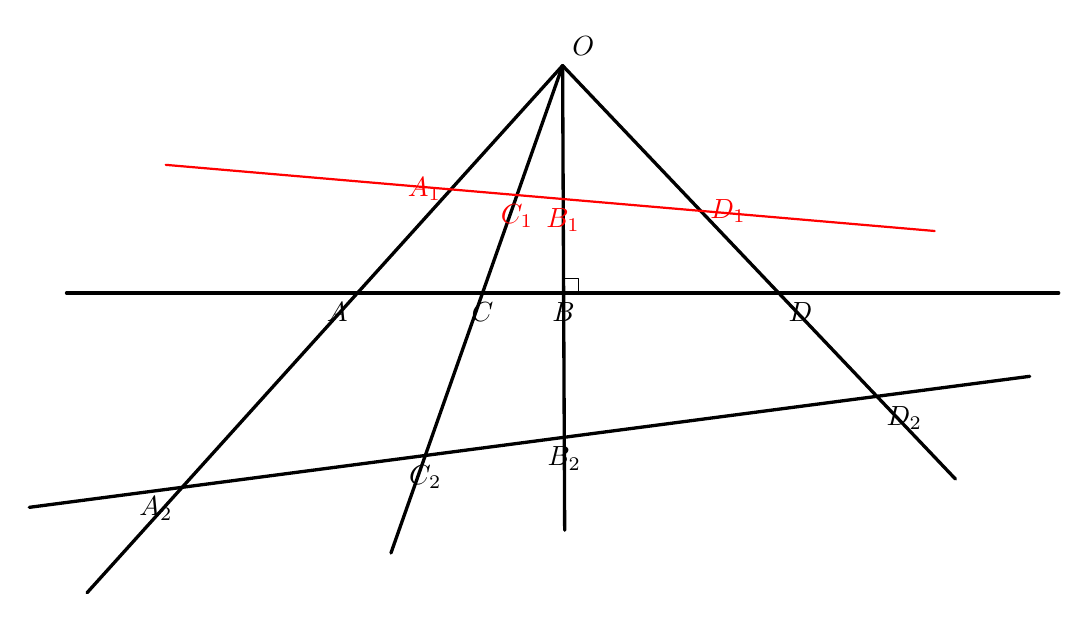
\begin{tikzpicture}[scale=1.05, line cap=round, line join=round]
			
			%====================
			% 1) 基本点与底边 A2D2（延长后的直线）
			%====================
			\coordinate (O)  at (0,4.2);
			
			% 先取底边上的两个基准点（用于确定底边方向）
			\coordinate (A2) at (-4.6,-0.9);
			\coordinate (D2) at ( 3.8, 0.2);
			
			% 在底边上再取两点，便于画出四线束
			\coordinate (B2) at ($(A2)!0.55!(D2)$);
			\coordinate (C2) at ($(A2)!0.35!(D2)$);
			
			% 将 A2D2 延长：在 A2->D2 方向上向两侧外推
			\def\tbase{0.22} % 延长比例，可调大/调小
			\coordinate (A2L) at ($(A2)!-\tbase!(D2)$);
			\coordinate (D2R) at ($(A2)!{1+\tbase}!(D2)$);
			
			% A2D2：画成延长线（无箭头）
			\draw[very thick] (A2L) -- (D2R);
			
			%====================
			% 2) 四条“射线”OA,OC,OB,OD：从 O 出发沿方向延长（不画箭头）
			%====================
			\def\k{1.25} % 射线延长倍数，可调
			\coordinate (A2e) at ($(O)!\k!(A2)$);
			\coordinate (C2e) at ($(O)!\k!(C2)$);
			\coordinate (B2e) at ($(O)!\k!(B2)$);
			\coordinate (D2e) at ($(O)!\k!(D2)$);
			
			\draw[very thick] (O) -- (A2e);
			\draw[very thick] (O) -- (C2e);
			\draw[very thick] (O) -- (B2e);
			\draw[very thick] (O) -- (D2e);
			
			%====================
			% 3) 中间水平截线：AD 也要延长（画成整条直线）
			%====================
			\path[name path=hline] (-6,1.45) -- (6,1.45);
			
			% 用延长后的射线来求交
			\path[name path=OA2] (O) -- (A2e);
			\path[name path=OC2] (O) -- (C2e);
			\path[name path=OB2] (O) -- (B2e);
			\path[name path=OD2] (O) -- (D2e);
			
			\path[name intersections={of=OA2 and hline, by=A}];
			\path[name intersections={of=OC2 and hline, by=C}];
			\path[name intersections={of=OB2 and hline, by=B}];
			\path[name intersections={of=OD2 and hline, by=D}];
			
			% AD：延长线（无箭头）
			\draw[very thick] (-6,1.45) -- (6,1.45);
			
			%====================
			% 4) 上方红色截线：产生 A1,C1,B1,D1
			%====================
			\path[name path=redline] (-4.8,3.0) -- (4.5,2.2);
			
			\path[name intersections={of=OA2 and redline, by=Aone}];
			\path[name intersections={of=OC2 and redline, by=Cone}];
			\path[name intersections={of=OB2 and redline, by=Bone}];
			\path[name intersections={of=OD2 and redline, by=Done}];
			
			\draw[thick, red] (-4.8,3.0) -- (4.5,2.2);
			
			%====================
			% 5) 点标注
			%====================
			\node[above right] at (O) {$O$};
			
			\node[below left]  at (A) {$A$};
			\node[below]       at (C) {$C$};
			\node[below]       at (B) {$B$};
			\node[below right] at (D) {$D$};
			
			\node[below left]  at (A2) {$A_2$};
			\node[below]       at (C2) {$C_2$};
			\node[below]       at (B2) {$B_2$};
			\node[below right] at (D2) {$D_2$};
			
			\node[left]  at (Aone) {\color{red}$A_1$};
			\node[below] at (Cone) {\color{red}$C_1$};
			\node[below] at (Bone) {\color{red}$B_1$};
			\node[right] at (Done) {\color{red}$D_1$};
			
			%====================
			% 6) 直角符号（示意）
			%====================
			\draw ($(B)+(0.18,0)$) -- ($(B)+(0.18,0.18)$) -- ($(B)+(0,0.18)$);
			
		\end{tikzpicture}
		
	\end{figure}
	
	\[
	\left(\frac{AC}{AB}\right)\Big/\left(\frac{BC}{BD}\right)
	\quad\text{之比，称为交比。}
	\]
	\textbf{1.\;交比具有射影不变性。}
	
	\medskip
	\noindent\textbf{（由面积比推出的交比表达式）}
	\[
	\left(\frac{AC}{AD}\right)\Big/\left(\frac{BC}{BD}\right)
	=
	\left(\frac{S_{\triangle AOC}}{S_{\triangle AOD}}\right)\Big/\left(\frac{S_{\triangle BOC}}{S_{\triangle BOD}}\right)
	\]
	
	\[
	=
	\left(\frac{\tfrac12\,OA\cdot OC\cdot\sin\angle AOC}{\tfrac12\,OA\cdot OD\cdot\sin\angle AOD}\right)
	\Bigg/
	\left(\frac{\tfrac12\,OC\cdot OB\cdot\sin\angle COB}{\tfrac12\,OD\cdot OB\cdot\sin\angle BOD}\right).
	\]
	
	
	\[
	=
	\left(\frac{\sin\angle AOC}{\sin\angle AOD}\right)\Big/\left(\frac{\sin\angle COB}{\sin\angle BOD}\right)
	=
	\frac{\sin\angle AOC}{\sin\angle AOD}\cdot\frac{\sin\angle BOD}{\sin\angle COB}.
	\]
	
	\medskip
	\noindent\textbf{二、当交比为 $-1$（调和比）}
	\[
	\overrightarrow{AC}=\lambda\,\overrightarrow{CB},\qquad
	\overrightarrow{AD}=-\lambda\,\overrightarrow{DB},
	\qquad (\lambda>0\ \text{且}\ \lambda\neq 1),
	\]
	\[
	\left|\frac{AC}{AD}\right|=\left|\frac{CB}{DB}\right|.
	\]
	
	\medskip
	\begin{center}
		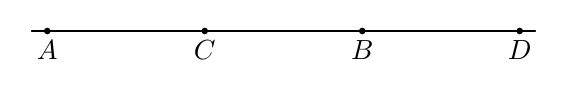
\begin{tikzpicture}[scale=1, line cap=round, line join=round]
			\draw (-0.2,0)--(6.2,0);
			\fill (0,0) circle (1.2pt) node[below] {$A$};
			\fill (2,0) circle (1.2pt) node[below] {$C$};
			\fill (4,0) circle (1.2pt) node[below] {$B$};
			\fill (6,0) circle (1.2pt) node[below] {$D$};
		\end{tikzpicture}
	\end{center}
	
	\noindent\textbf{$A,C,B,D$ 调和点列：}
	\begin{enumerate}
		\item $A,B$ 为基点，$C,D$ 为内外分点，$CD$ 调和分割 $AB$。
		\item $C,D$ 为基点，$B,A$ 为内外分点，$AB$ 调和分割 $CD$。
		\item $AB,\,CD$ 调和共轭。
	\end{enumerate}
	
	\medskip
	\noindent\textbf{3.}\quad
	\[
	\frac{2}{AB}=\frac{1}{AC}+\frac{1}{AD}.
	\]
	\noindent 记：
	\[
	\frac{BC}{AC}=\frac{BD}{AD}.
	\]
	\[
	\frac{AB-AC}{AC}=\frac{AD-AB}{AD}
	\quad\Longrightarrow\quad
	\frac{AB}{AC}-1=1-\frac{AB}{AD}
	\]
	\[
	\Longrightarrow\quad
	\frac{AB}{AC}+\frac{AB}{AD}=2
	\quad\Longrightarrow\quad
	\frac{1}{AC}+\frac{1}{AD}=\frac{2}{AB}.
	\]
	
	% =========================
	
	\begin{tikzpicture}[scale=1.5, thick]
		% 定义顶点 O
		\coordinate (O) at (0,3);
		\node[above] at (O) {$O$};
		
		% 定义底部的四条射线
		\coordinate (A_inf) at (-2,0);
		\coordinate (C_inf) at (-0.8,0);
		\coordinate (B_inf) at (0.5,0);
		\coordinate (D_inf) at (2,0);
		
		% 画射线
		\draw[red] (O) -- (-2.5,-0.5);
		\draw[red] (O) -- (-1,-0.5);
		\draw[red] (O) -- (0.8,-0.5);
		\draw[red] (O) -- (2.5,-0.5);
		
		% 画第一条截线 (底部)
		\draw[red] (-2,0.5) -- (2,0.5);
		\coordinate (A) at (-1.5,0.5);
		\coordinate (C) at (-0.6,0.5);
		\coordinate (B) at (0.4,0.5);
		\coordinate (D) at (1.4,0.5);
		
		\node[below left, red] at (A) {$A$};
		\node[below, red] at (C) {$C$};
		\node[below, red] at (B) {$B$};
		\node[below right, red] at (D) {$D$};
		
		% 画第二条斜截线 (蓝色)
		\draw[blue] (-2.2,0.8) -- (1.5,2.2);
		\coordinate (Ap) at (-1.1,1.2);
		\coordinate (Cp) at (-0.35,1.5);
		\coordinate (Bp) at (0.2,1.7);
		\coordinate (Dp) at (0.55,1.85);
		
		\node[below, blue] at (Ap) {$A'$};
		\node[below, blue] at (Cp) {$C'$};
		\node[below, blue] at (Bp) {$B'$};
		\node[right, blue] at (Dp) {$D'$};
		
		% 文字标注
		\node[align=left, anchor=west] at (-1.5,4) {
			\textbf{\underline{调和点列}} $\left\{ 
			\begin{array}{l}
				1. \text{交比为 } -1 \text{ (调和平均)} \\
				2. \text{射影不变性}
			\end{array} \right.$
		};
	\end{tikzpicture}	
	
	\begin{tikzpicture}[thick, scale=1.2]
		
		% 1. 定义核心顶点 (P 和 Q)
		\coordinate (P) at (0,0);
		\coordinate (Q) at (6,8);
		
		% 2. 定义从 Q 发出的两条主干线 (蓝线)
		\path[name path=lineQ1] (Q) -- (3,-1);
		\path[name path=lineQ2] (Q) -- (9,-1);
		
		% 3. 定义 P 发出的顶部和底部射线 (用于确定 A, B, C, D)
		\path[name path=rayTop] (P) -- (10,5);   % 经过 A, E, D
		\path[name path=rayBot] (P) -- (10,0.8); % 经过 B, F, C
		
		% 4. 计算交点 A, B, C, D
		\fill [name intersections={of=lineQ1 and rayTop, by=A}] (A) circle (1.5pt) node[left] {$A$};
		\fill [name intersections={of=lineQ1 and rayBot, by=B}] (B) circle (1.5pt) node[below left] {$B$};
		\fill [name intersections={of=lineQ2 and rayTop, by=D}] (D) circle (1.5pt) node[right] {$D$};
		\fill [name intersections={of=lineQ2 and rayBot, by=C}] (C) circle (1.5pt) node[right] {$C$};
		
		% 5. 绘制对角线并确定点 O
		\draw[blue, thin] (A) -- (C);
		\draw[blue, thin] (B) -- (D);
		\path[name path=diagAC] (A) -- (C);
		\path[name path=diagBD] (B) -- (D);
		\fill [name intersections={of=diagAC and diagBD, by=O}] (O) circle (2pt) node[below right, red] {$O$};
		
		% 6. 【核心修改】定义射线 P-G-O-H，确保其经过 O
		% 使用 ($ (P)!1.5!(O) $) 来延长线段，确保覆盖到 H 点所在的区域
		\path[name path=rayMid] (P) -- ($(P)!1.8!(O)$); 
		
		% 计算 G 和 H (射线与 Q 发出的蓝线的交点)
		\fill [name intersections={of=lineQ1 and rayMid, by=G}] (G) circle (1.5pt) node[below left] {$G$};
		\fill [name intersections={of=lineQ2 and rayMid, by=H}] (H) circle (1.5pt) node[right] {$H$};
		
		% 7. 绘制穿过 Q 和 O 的中心线，并寻找 E 和 F
		\draw[name path=vertLine] ($(Q)!-0.2!(O)$) -- ($(Q)!1.5!(O)$);
		\node[right] at (Q) {$Q$};
		\fill [name intersections={of=vertLine and rayTop, by=E}] (E) circle (1.5pt) node[above left] {$E$};
		\fill [name intersections={of=vertLine and rayBot, by=F}] (F) circle (1.5pt) node[below left] {$F$};
		
		% 8. 绘制所有实线 (移除所有箭头)
		\draw[red] (P) -- (D); % 顶部红线
		\draw[black] (P) -- (H); % 中间线 (经过 G, O, H)
		\draw[red] (P) -- (C); % 底部红线
		
		\draw (A) -- (D); % 横线
		\draw (B) -- (C); % 横线
		
		\draw[blue] (Q) -- (B); % Q发出的左侧蓝线
		\draw[blue] (Q) -- (C); % Q发出的右侧蓝线
		
		% 标注顶点 P
		\node[below left] at (P) {$P$};
		
	\end{tikzpicture}
	
	
	\begin{tikzpicture}[thick, scale=1.1, font=\small]
		
		% --- 1. 定义核心坐标 ---
		% 顶点 O 位于右上方
		\coordinate (O) at (8, 6);
		% 截线的高度（y坐标）
		\def\lineY{2}
		% 定义垂足 H
		\coordinate (H) at (8, \lineY);
		
		% --- 2. 绘制水平截线 (红线) ---
		\draw[red, line width=0.8pt] (0, \lineY) -- (10, \lineY);
		\node[red, below right] at (6.5, \lineY) {调和点列};
		
		% --- 3. 计算并绘制线束 ---
		% 根据图中比例，手动设定 A, B, C, D 的横坐标
		\coordinate (A) at (1, \lineY);
		\coordinate (B) at (3.5, \lineY);
		\coordinate (C) at (5.5, \lineY);
		\coordinate (D) at (7, \lineY);
		
		% 绘制四条线束 (蓝线)
		\draw[blue] (O) -- ($(O)!1.2!(A)$);
		\draw[blue] (O) -- ($(O)!1.2!(B)$);
		\draw[blue] (O) -- ($(O)!1.2!(C)$);
		\draw[blue] (O) -- ($(O)!1.2!(D)$);
		
		% --- 4. 标注点与斜率标识 ---
		% 顶点 O
		\fill[blue] (O) circle (1.5pt) node[right, black] {$O$};
		
		% 交点 A, B, C, D
		\foreach \p in {A,B,C,D} {
			\fill[red] (\p) circle (1.5pt);
			\node[below left, black] at (\p) {$\p$};
		}
		
		% 标注 k1, k2, k3, k4
		\node[above left] at ($(O)!0.6!(A)$) {$k_1$};
		\node[above left] at ($(O)!0.6!(B)$) {$k_2$};
		\node[above left] at ($(O)!0.5!(C)$) {$k_3$};
		\node[left] at ($(O)!0.5!(D)$) {$k_4$};
		
		% --- 5. 绘制垂直高度 h ---
		\draw[dashed, red] (O) -- (H);
		\fill[black] (H) circle (1.2pt) node[below] {$H$};
		\node[right] at ($(O)!0.5!(H)$) {$h$};
		
		% --- 6. 旁边的文字标注 (可选) ---
		\node[anchor=west, align=left] at (9, 5) {
			$OA, OB, OC, OD$ \\
			\textbf{调和线束}
		};
		
		% 底部的调和比公式还原
		\node[below] at (3.5, 0.5) {$\displaystyle \frac{AB}{AD} = \frac{BC}{CD}$};
		
	\end{tikzpicture}
	
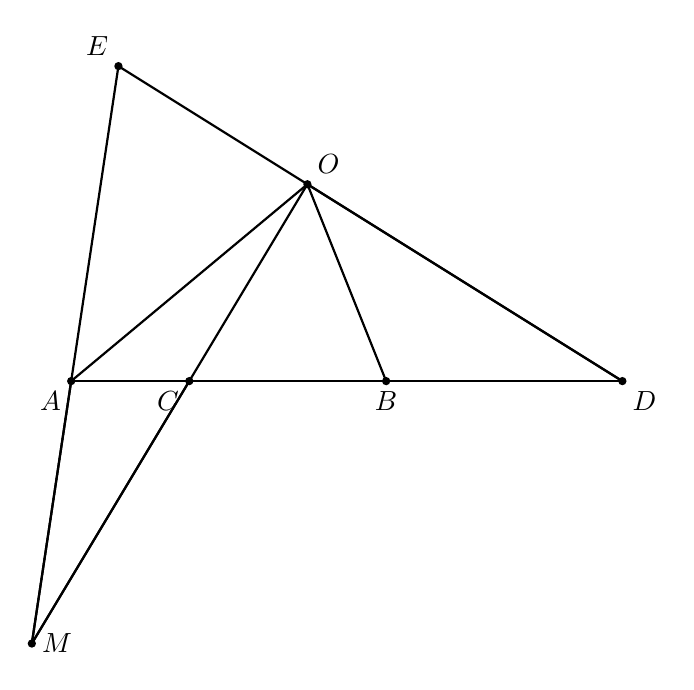
\begin{tikzpicture}[line join=round, line cap=round, thick]
	
	% --- 1. 定义核心坐标 ---  
	% 设定基线上的点 (根据图片比例调整)
	\coordinate (A) at (0,0);
	\coordinate (C) at (1.5,0);
	\coordinate (B) at (4,0);
	\coordinate (D) at (7,0);
	
	% 设定顶点 O
	\coordinate (O) at (3,2.5);
	
	% --- 2. 满足 E, O, D 三点共线 ---
	% 使用 calc 库或者简单的位似变换，让 E 落在 DO 的延长线上
	% 这里将 E 设定在从 D 穿过 O 之后的一段距离
	\coordinate (E) at ($(D)!1.6!(O)$); 
	
	% --- 3. 计算交点 M ---
	% M 是直线 EA 和直线 OC 的交点
	\coordinate (M) at (intersection of E--A and O--C);
	
	% --- 4. 绘制直线 ---
	% 绘制基线
	\draw (A) -- (D);
	
	% 绘制从 O 发出的线束
	\draw (O) -- (A);
	\draw (O) -- (B);
	\draw (O) -- (D); % 这条线实际上包含了线段 EO
	\draw (O) -- (M); % 这条线包含了 OC
	
	% 绘制从 E 发出的线
	\draw (E) -- (M); % 这条线包含了 EA
	\draw (E) -- (D); % 明确连接 E, O, D 的共线长线
	
	% 为了还原图片中 M 在下方的视觉效果，稍微延长线段
	\draw (A) -- (M);
	\draw (C) -- (M);
	
	% --- 5. 标注节点 ---
	% 这里的标记位置根据图片视觉进行了微调
	\fill (A) circle (1.5pt) node[below left] {$A$};
	\fill (B) circle (1.5pt) node[below] {$B$};
	\fill (C) circle (1.5pt) node[below left] {$C$};
	\fill (D) circle (1.5pt) node[below right] {$D$};
	\fill (O) circle (1.5pt) node[above right] {$O$};
	\fill (E) circle (1.5pt) node[above left] {$E$};
	\fill (M) circle (1.5pt) node[right] {$M$};
	
\end{tikzpicture}
	
	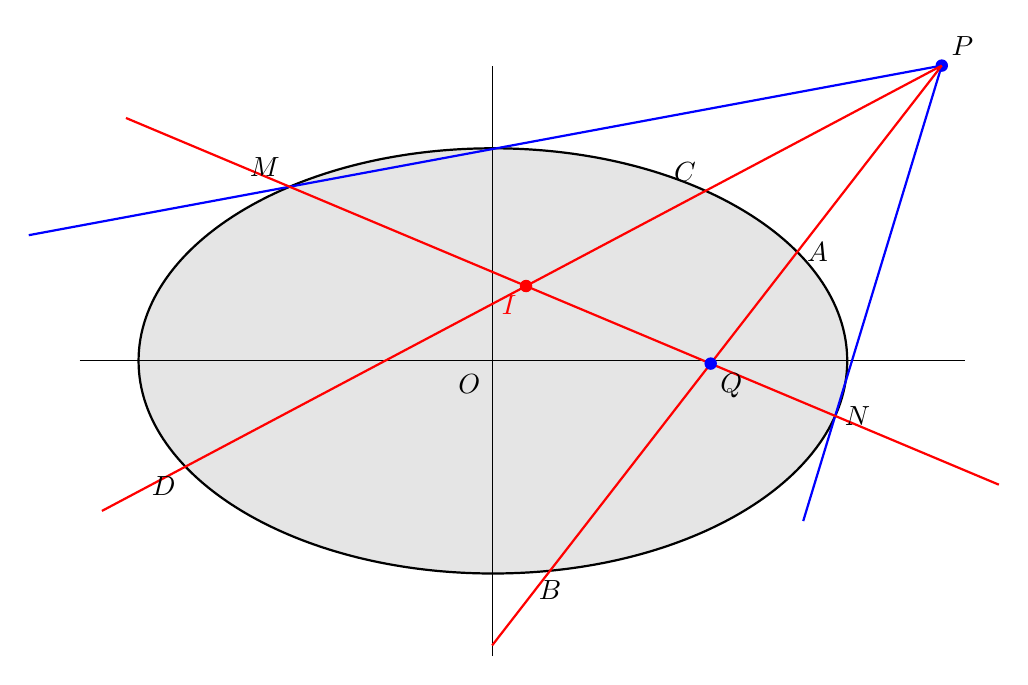
\begin{tikzpicture}[scale=1.5]
		% 0. 需在导言区引用：\usetikzlibrary{intersections, calc}
		
		% 1. 绘制灰色填充的椭圆
		\def\ea{3} \def\eb{1.8}
		\fill[gray!20] (0,0) ellipse ({\ea} and {\eb});
		\draw[thick, name path=ellipse] (0,0) ellipse ({\ea} and {\eb});
		
		% 2. 绘制坐标轴 (保留轴线，去掉箭头和标注)
		\draw (-3.5,0) -- (4,0);
		\draw (0,-2.5) -- (0,2.5);
		\node at (-0.2,-0.2) {$O$};
		
		% 3. 定义切点 M 和 N，并由切线交点确定极点 P
		\coordinate (M) at ({3*cos(125)}, {1.8*sin(125)});
		\coordinate (N) at ({3*cos(-15)}, {1.8*sin(-15)});
		
		% P点位置
		\coordinate (P) at (3.8, 2.5); 
		
		% 绘制蓝色切线 (PM 和 PN)
		\draw[blue, thick] (P) -- ($(P)!1.4!(M)$);
		\draw[blue, thick] (P) -- ($(P)!1.3!(N)$);
		\node[above right] at (P) {$P$};
		\fill[blue] (P) circle (1.5pt);
		
		% 4. 绘制红色极线 MN
		\draw[red, thick, name path=lineMN] ($(M)!-0.3!(N)$) -- ($(N)!-0.3!(M)$);
		\node[above left] at (M) {$M$};
		\node[right] at (N) {$N$};
		
		% 5. 绘制穿过 P 的两条红色割线，并向外延长
		% 割线1: P-C-D (向D点后延长)
		\path[name path=pathPD] (P) -- (-2.8, -1.0);
		\draw[red, thick, name intersections={of=ellipse and pathPD, by={C,D}}] 
		(P) -- ($(D)!-0.8cm!(P)$);
		\node[above left] at (C) {$C$};
		\node[below left] at (D) {$D$};
		
		% 割线2: P-A-B (向B点后延长)
		\path[name path=pathPB] (P) -- (0.0, -2.4);
		\draw[red, thick, name intersections={of=ellipse and pathPB, by={A,B}}] 
		(P) -- ($(B)!-0.8cm!(P)$);
		\node[right] at (A) {$A$};
		\node[below] at (B) {$B$};
		
		% 6. 计算并标注交点 I 和 Q (严格交于极线 MN)
		\path [name intersections={of=pathPD and lineMN, by={I}}];
		\fill[red] (I) circle (1.5pt) node[below left] {$I$};
		
		% Q 是直线 PB 与 极线 MN 的交点
		\path [name intersections={of=pathPB and lineMN, by={Q}}];
		\fill[blue] (Q) circle (1.5pt) node[below right, black] {$Q$};
		
	\end{tikzpicture}
	
	
	%%%%%%%%%%%%%%%
	\begin{tikzpicture}[scale=1.2, >=stealth]
		% 1. 画布裁剪
		\clip (-3.5, -3) rectangle (5.5, 3.5);
		
		\def\a{2.5}
		\def\b{1.5}
		
		% 2. 坐标轴
		\draw[->, gray!50, thin] (-3.2,0) -- (5,0) node[right] {$x$};
		\draw[->, gray!50, thin] (0,-2.5) -- (0,3) node[above] {$y$};
		
		% 3. 椭圆
		\draw[thick, red, name path=ellipse] (0,0) circle [x radius=\a, y radius=\b];
		\fill[red, opacity=0.05] (0,0) circle [x radius=\a, y radius=\b];
		
		% 4. 设定点 P
		\coordinate (P) at (3.5, 2.5); 
		\fill[red] (P) circle (1.5pt) node[above right] {$P$};
		
		% 5. 构造割线并命名路径 (延长路径确保能与极线相交)
		\path[name path=linePAB] (P) -- ($(P)!1.8!(-2, -1.2)$);
		\path [name intersections={of=ellipse and linePAB, by={A,B}}];
		\draw[blue!70, thin] (P) -- (B);
		
		\path[name path=linePCD] (P) -- ($(P)!1.8!(0.5, -2.5)$);
		\path [name intersections={of=ellipse and linePCD, by={C,D}}];
		\draw[blue!70, thin] (P) -- (D);
		
		% 6. 计算交点 M 和 N
		\coordinate (N) at (intersection of A--D and B--C);
		\coordinate (M) at (intersection of A--C and B--D);
		
		% 7. 绘制极线 MN (定义为 path 以便求交点)
		\def\ext{2.5} % 延伸系数
		\path[name path=polarLine] ($(M)!\ext!(N)$) -- ($(N)!\ext!(M)$);
		\draw[orange, thick] ($(M)!\ext!(N)$) -- ($(N)!\ext!(M)$) node[below] {极线 $l$};
		
		% 8. --- 关键修正：计算 E 和 F ---
		% E 是极线与割线 PAB 的交点
		\fill [name intersections={of=polarLine and linePAB, by={E}}] (E) circle (1.5pt) node[left, xshift=-2pt] {$E$};
		
		% F 是极线与割线 PCD 的交点
		\fill [name intersections={of=polarLine and linePCD, by={F}}] (F) circle (1.5pt) node[below right] {$F$};
		
		% 9. 绘制辅助线
		\draw[black, dashed] (A) -- (D);
		\draw[black, dashed] (B) -- (C);
		\draw[black] (A) -- (M); 
		\draw[black] (B) -- (M); 
		
		% 10. 标注剩余点
		\fill (N) circle (1.5pt) node[below left] {$N$};
		\fill (M) circle (1.5pt) node[right, xshift=2pt] {$M$};
		
		\node[above] at (A) {$A$};
		\node[left] at (B) {$B$};
		\node[right] at (C) {$C$};
		\node[below] at (D) {$D$};
		
	\end{tikzpicture}
\end{document}
